En ``Carlimpio'' el tiempo de lavado del auto puede modelarse como un proceso de Poisson con una media de 12 autos por hora.
% Es Exponencial porque es un proceso entre dos eventos Poisson
% lambda = 12 autos/hora = 0.2 autos/min
% teta = 1/lambda = 5 min/auto
% aa me enrede xD
\begin{itemize}
	\item ?`Cu\'al es la esperanza y varianza de tiempo de lavado por auto en minutos?\\
		$Esperanza\ =\ E(x)\ =\ \frac{1}{\lambda}\ =\ 5$\\
		$Varianza\ =\ V(x)\ =\ \frac{1}{\lambda^2}\ =\ 25$\\
	\item ?`Cu\'al es la probabilidad de que se demore m\'as de 8 minutos en lavar un auto?\\
		$P(X>8)\ =\ 1\ -\ P(X<8)\ =\ 1\ -\ 0.7981035\ =\ 0.2018965\ $\\
	\item ?`Cu\'al es la probabilidad de que el tiempo de lavado de un auto sea menor que 10 minutos dado que lleva 4 minutos lav\'andose?\\
		 % si lleva 4 minutos, entonces le falta 1 minuto aproximadamente, entonces seria P(4<X<10) ?    
                $P(4< X < 10) = P(X < 10)\ -\ P(X < 4) = 0.3139937$\\ % pexp(10,0.2)-pexp(4,0.2)
	\item Realice gr\'aficos de la funci\'on de densidad de probabilidad y de la funci\'on de distribuci\'on.\\
		Funci\'on de distribuci\'on:\\
                  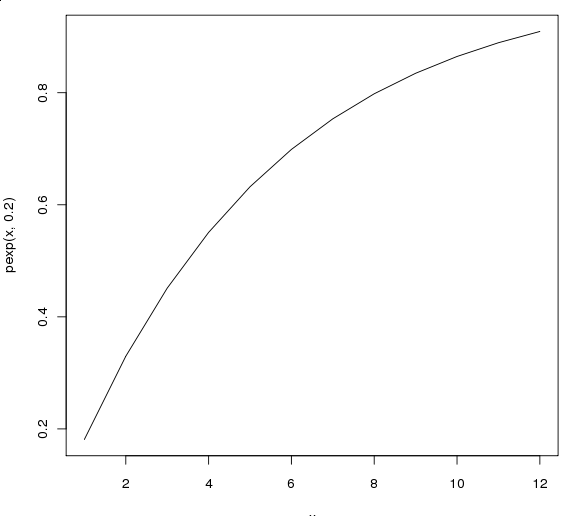
\includegraphics[width=3.3in,height=3.3in]{images/2_3-pexp}\\% plot(x,pexp(x,0.2),type="l") %Distribucion
                Funci\'on de densidad de probabilidad:\\
                  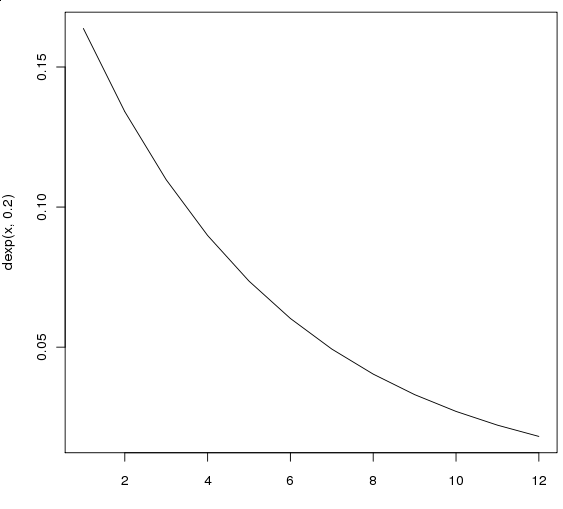
\includegraphics[width=3.3in,height=3.3in]{images/2_3-dexp}\\% plot(x,dexp(x,0.2),type="l") %Densidad
	\item Var\'ie el o los valores de los par\'ametros de la distribuci\'on y comente lo observado en los gr\'aficos de la funci\'on de densidad y de distribuci\'on. (2 casos).\\
	\begin{itemize}
		\item Funcion de densidad\\
		Variando lambda (0.5):\\
		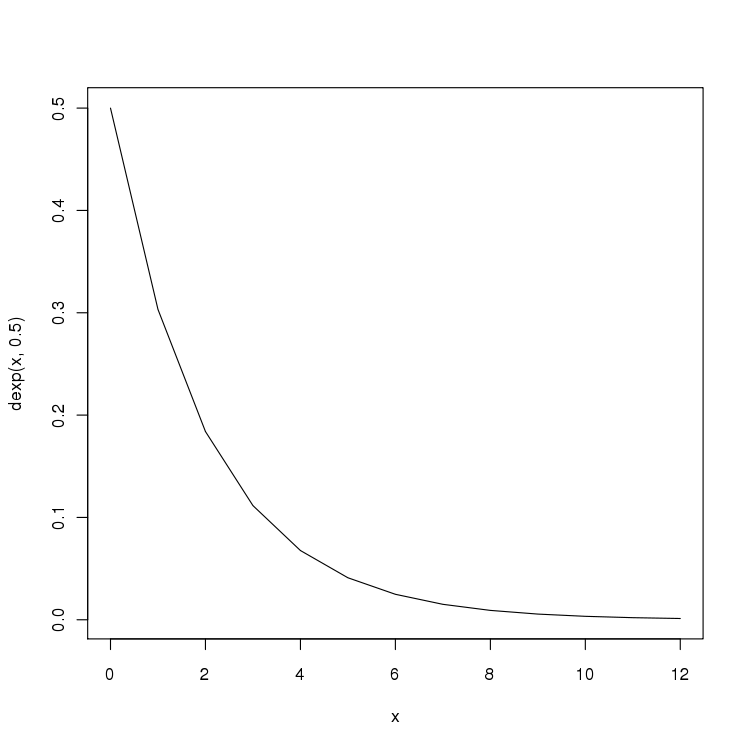
\includegraphics[width=3.3in,height=3.3in]{images/2_3-dexp-variado1}\\
		Variando lambda (0.8):\\
                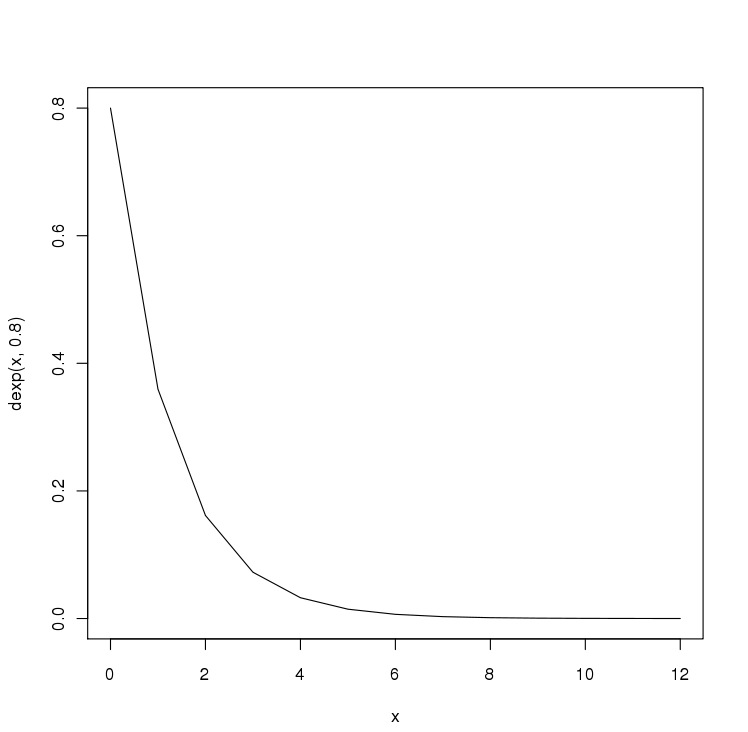
\includegraphics[width=3.3in,height=3.3in]{images/2_3-dexp-variado2}\\
		Claramente, y juzgando por la forma de la funci\'on, al obtener valores de lambda cercanos a 1, la funci\'on se acerca a la exponencial.\\
	\item Funcion de Distribucion\\
                Variando lambda (0.5):\\
                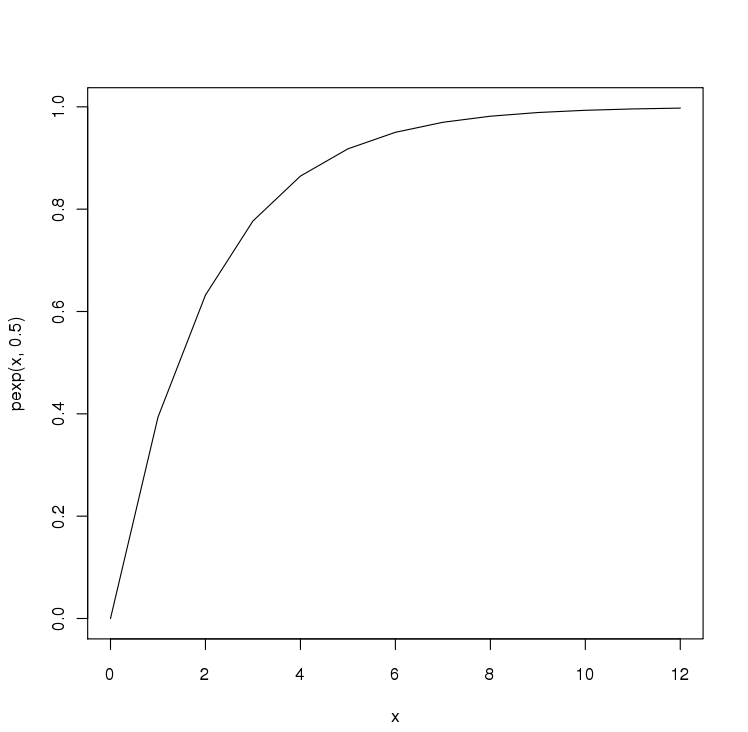
\includegraphics[width=3.3in,height=3.3in]{images/2_3-pexp-variado1}\\
                Variando lambda (0.8):\\
                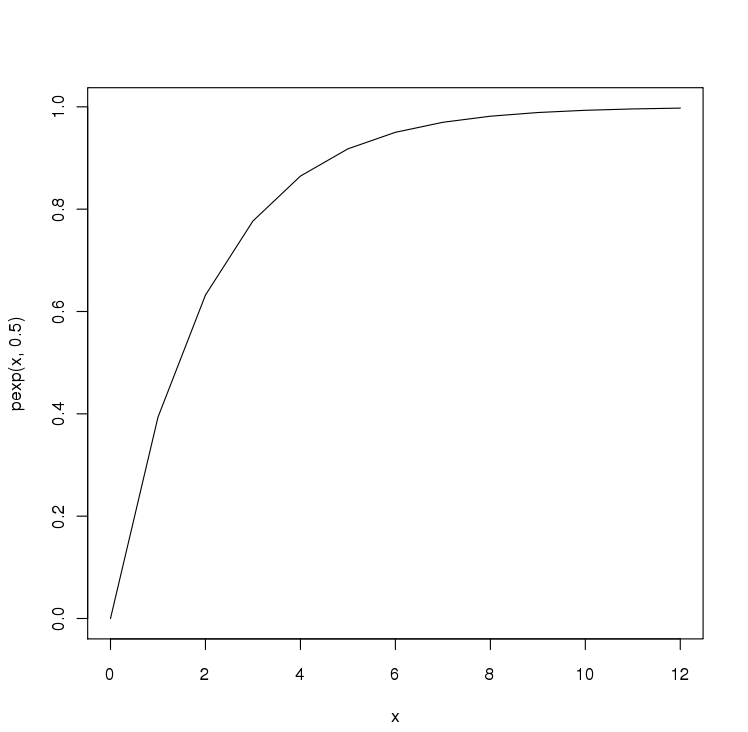
\includegraphics[width=3.3in,height=3.3in]{images/2_3-pexp-variado2}\\
                Al igual que en el caso anterior, al obtener valores de lambda cercanos a
1, la funci\'on se acerca a la funci\'on exponencial.\\


	\end{itemize}
\end{itemize}
